% file: DeepSVM.tex
%
% github        : ernestyalumni
% gmail         : ernestyalumni 
% linkedin      : ernestyalumni 
% wordpress.com : ernestyalumni
%
% This code is open-source, governed by the Creative Common license.  Use of this code is governed by the Caltech Honor Code: ``No member of the Caltech community shall take unfair advantage of any other member of the Caltech community.'' 

\documentclass[10pt]{amsart}
\pdfoutput=1
\usepackage{mathtools,amssymb,lipsum,caption}

\usepackage{graphicx}
\usepackage{hyperref}
\usepackage[utf8]{inputenc}
\usepackage{listings}
\usepackage[table]{xcolor}
\usepackage{pdfpages}
\usepackage{tikz}
\usetikzlibrary{matrix,arrows}

\usepackage{breqn} % for dmath


\usepackage{cancel} % for Feynman slash notation

\hypersetup{colorlinks=true,citecolor=[rgb]{0,0.4,0}}


%\oddsidemargin=15pt
%\evensidemargin=5pt
%\hoffset-45pt
%\voffset-55pt
%\topmargin=-4pt
%\headsep=5pt
%\textwidth=1120pt
%\textheight=595pt
%\paperwidth=1200pt
%\paperheight=700pt
%\footskip=40pt








\newtheorem{theorem}{Theorem}
\newtheorem{corollary}{Corollary}
%\newtheorem*{main}{Main Theorem}
\newtheorem{lemma}{Lemma}
\newtheorem{proposition}{Proposition}

\newtheorem{definition}{Definition}
\newtheorem{remark}{Remark}

\newenvironment{claim}[1]{\par\noindent\underline{Claim:}\space#1}{}
\newenvironment{claimproof}[1]{\par\noindent\underline{Proof:}\space#1}{\hfill $\blacksquare$}

%This defines a new command \questionhead which takes one argument and
%prints out Question #. with some space.
\newcommand{\questionhead}[1]
  {\bigskip\bigskip
   \noindent{\small\bf Question #1.}
   \bigskip}

\newcommand{\problemhead}[1]
  {
   \noindent{\small\bf Problem #1.}
   }

\newcommand{\exercisehead}[1]
  { \smallskip
   \noindent{\small\bf Exercise #1.}
  }

\newcommand{\solutionhead}[1]
  {
   \noindent{\small\bf Solution #1.}
   }


  \title[Deep Support Vector Machines (SVM)]{Deep Support Vector Machines (SVM)}

\author{Ernest Yeung \href{mailto:ernestyalumni@gmail.com}{ernestyalumni@gmail.com}}
\date{5 avril 2017}
\keywords{Machine Learning, Support Vector Machines, Neural Networks, Deep Neural Networks, Constrained Optimization, Projected Gradient Descent, CUDA C/C++, theano}

\begin{document}

\definecolor{darkgreen}{rgb}{0,0.4,0}
\lstset{language=Python,
 frame=bottomline,
 basicstyle=\scriptsize,
 identifierstyle=\color{blue},
 keywordstyle=\bfseries,
 commentstyle=\color{darkgreen},
 stringstyle=\color{red},
 }
%\lstlistoflistings

\maketitle

\tableofcontents

%\begin{multicols*}{2}


 











\begin{abstract}
\section{Executive Summary}
\end{abstract}


\section{Right $R$-modules}

Consider, as a start, the total given (training) input data, consisting of $m\in \mathbb{Z}^+$ (training) examples, each example, say the $i$th example, being represented by a "feature" vector of $d$ features, $X^{(i)} \in \mathbb{K}^d$, where $\mathbb{K}$ is a field or (categorical) classes, i.e. as examples of fields, the real numbers $\mathbb{R}$, or integers $\mathbb{Z}$, so that $\mathbb{K} = \mathbb{R},\mathbb{Z}$ or $\mathbb{K} = \lbrace 0 ,1,\dots K-1\rbrace$, where $K$ is the total number of classes that a feature could fall into.  Note that for this case, the case of $\mathbb{K}=\lbrace 0 ,1,\dots K-1\rbrace$, for $K$ classes, though labeled by integers, this set of integer labels is \emph{not} equipped with ordered field properties (it is meaningless to say $0<1$, for example), nor the usual field (arithmetic) operations (you cannot add, subtract, multiply, or even take the modulus of these integers).  How can we "feed into" our machine such (categorical) class data?  Possibly, we should intuitively think of the Kronecker Delta function:
\[
\delta_{iJ} = \begin{cases} 0 & \text{ if } i\neq J \\ 
 1 & \text{ if } i = J \end{cases}
\]
for some (specific) class $J$, represented by an integer.  So perhaps our machine can learn kronecker delta, or "signal"-like functions that will be "activated" if the integer value of a piece (feature) of data is exactly equal to $J$ and $0$ otherwise.  

Onward, supposing $\mathbb{K}$ is a field, consider the total given input data of $m$ examples:
\[
\lbrace X^{(i)} \in \mathbb{K}^d\rbrace^m_{i=1,2,\dots m}
\]
One can arrange such input data into a $m\times d$ matrix.  We want to do this, for one reason, to \emph{take advantage of the parallelism afforded by GPU(s)}.  Thus we'd want to act upon the entire input data set $\lbrace X^{(i)} \in \mathbb{K}^d\rbrace^m_{i=1,2,\dots m}$.  

We'd also want to do \emph{parallel reduce} in order to do a \emph{summation}, $\sum_{i=1}^m$, over all (training) examples, to obtain a cost function(al) $J$.  

For \verb|theano|, parallel \verb|reduce| and \verb|scan| operations can only be done over the first dimension of a \verb|theano| tensor.  Thus, we write the total input data as such:
\begin{equation}
\lbrace X^{(i)} \in \mathbb{K}^d\rbrace^m_{i=1,2,\dots m} \mapsto X^{(i)}_j \in \text{Mat}_{\mathbb{K}}(m,d)
\end{equation}
i.e. $X^{(i)}_j$ is a $m\times d$ matrix of $\mathbb{K}$ values, with each $i$th row corresponding to the $i=1,2,\dots m$th example,  and $j$th column corresponding to the $j=1,2,\dots d$th feature (of the feature vector $X^{(i)} \in \mathbb{K}^d$).  

Let's, further, make the following abstraction, in that the input data $\lbrace X^{(i)} \in \mathbb{K}^d\rbrace^m_{i=1,2,\dots m}$ is really an element of a right $R$-module $\mathbf{X}$, in the category of right $R$-modules $\text{\textbf{Mod}}_R$ with ring $R$, $R$ not necessarily being commutative.  

A reason for this abstraction is that if we allow the underlying ring $R$ to be a field $\mathbb{K}$, (e.g. $\mathbb{K}=\mathbb{R},\mathbb{Z}$), then the "usual" scalar multiplication by scalars is recovered.  But we also need to equip $X\in \text{\textbf{Mod}}_R$ with a \emph{right action}, where ring $R$ is \emph{noncommutative}, namely 
\[
R = \text{Mat}_{\mathbb{K}}(d,s) \cong L(\mathbb{K}^d, \mathbb{K}^s)
\]
where $\text{Mat}_{\mathbb{K}}(d,s)$ denotes the ring of all matrices over field $\mathbb{K}$ of matrix (size) dimensions $d\times s$ (it has $d$ rows and $s$ columns), $\cong$ is an isomorphism, $L(\mathbb{K}^d,\mathbb{K}^s)$ is the space of all (linear) maps from $\mathbb{K}^d$ to $\mathbb{K}^s$.  If $\mathbb{K}$ is a field, this isomorphism exists.  

Thus, for 
\begin{equation}
\begin{aligned}
	& X\in \mathbf{X} \in \text{Mod}_R \\
	&  R = \text{Mat}_{\mathbb{K}}(d,s) \cong L(\mathbb{K}^d,\mathbb{K}^s)
\end{aligned}
\end{equation}
Let $\Theta \in R$. $\Theta$ is also known as the "parameters" or "weights" (and is denoted by $w$ or $W$ by others).  

Consider, as a first (pedagogical) step, only a single example ($m=1$).  $X$ is only a single feature vector, $X\in \mathbb{K}^d$.  Then for basis $\lbrace e_{\mu} \rbrace_{\mu=1\dots d}$ of $\mathbb{K}^d$, corresponding dual basis $\lbrace e^{\mu} \rbrace_{\mu=1\dots d}$ (which is a basis for dual space $(\mathbb{K}^d)^*$), then
\[
\begin{gathered}
	X\Theta = X^{\mu} e_{\mu} ( \Theta^{\, \, \, j}_{  \nu} e_j \otimes e^{\nu}) =  \qquad \quad \, \begin{aligned} & \mu , \nu = 1 \dots d \\ 
&  j = 1\dots s \end{aligned} \\
X^{\mu} \Theta^{\, \, \, j}_{  \nu} e_j \otimes e^{\nu}(e_{\mu})  = X^{\mu} \Theta^{\, \, \, j}_{  \nu} e_j \delta^{\nu}_{\mu} = X^{\mu} \Theta^{\, \, \,  j}_{ \mu} e_j
\end{gathered}
\]
In this case where $X$ is simply a vector, one could think of $X$ as a "row matrix" and $\Theta$ is a matrix, acting on the right, in matrix multiplication.    

Now suppose, in general, $X \in \textbf{X} \in \text{\textbf{Mod}}_R$, where $X$ could be a $m\times d$ matrix, or higher-dimensional tensor.  For a concrete example, say $\textbf{X} = \text{Mat}_{\mathbb{K}}(m,d)$.  We not only have to equip this right $R$-module with the usual scalar multiplication, setting ring $R=\mathbb{K}$, but also the right action version of matrix multiplication, so that $R = \text{Mat}_{\mathbb{K}}(d,s)$.  This $R$ is \emph{non-commutative}, thus, necessitating the abstraction to right $R$-modules.  

Indeed, for
\[
\begin{gathered}
	\Theta \in L( \text{Mat}_{\mathbb{K}}(m,d), \text{Mat}_{\mathbb{K}}(m,s) ) \cong    (\text{Mat}_{\mathbb{K}}(m,d))^* \otimes \text{Mat}_{\mathbb{K}}(m,s) \cong \text{Mat}_{\mathbb{K}}(d,s), \text{ and so } \\
%	\Theta \cong w\otimes \alpha, \quad \, w \in   \text{Mat}_{\mathbb{K}}(m,s), \, \alpha \in (\text{Mat}_{\mathbb{K}}(m,d))^*, \text{ then } \\ 
%X\Theta = X w\otimes \alpha = w \otimes \alpha(X) = w \alpha(X) \in \text{Mat}_{\mathbb{K}}(m,s)
X\Theta \in \text{Mat}_{\mathbb{K}}(m,s)
\end{gathered}
\]
%with 
%\[
%\begin{gathered}
%	\alpha(X) \in \text{Mat}_{\mathbb{K}}(d,s)  \\ 
%\end{gathered}
%\]
Further
\[
X\Theta \in \text{Mat}_{\mathbb{K}}(m,s) \in \text{\textbf{Mod}}_R
\]
with ring $R$ in this case being $R=\text{Mat}_{\mathbb{K}}(s,s_2) \cong L(\mathbb{K}^s, \mathbb{K}^{s_2})$.  

Since $X\Theta$ is an element in a $R$-module, it is an element in an (additive) abelian group.  We can add the "intercept vector" $b$ (in theano, it'd be the usual theano vector, but with its dimensions "broadcasted" for all $m$ examples, i.e. for all $m$ rows).  
\[
X\Theta + b \in \text{Mat}_{\mathbb{K}}(m,s)
\]
Considering these 2 operatons on $X$, the "matrix multiplication on the right" or right action $\Theta$, and addition by $b$ together, through \emph{composition}, $(\Theta,b)$, we essentially have
\begin{equation}
X\in \mathbf{X} \in \text{\textbf{Mod}}_{R_1} \xrightarrow{ (\Theta,b) } X\Theta + b \in \mathbf{X_2} \in \text{\textbf{Mod}}_{R_2} 
\end{equation}
where
\[
\begin{aligned}
& R_1 = \text{Mat}_{\mathbb{K}}(d,s_1) \cong L(\mathbb{K}^d, \mathbb{K}^{s_1} ) \\ 
& R_2 = \text{Mat}_{\mathbb{K}}(s_1,s_2) \cong L(\mathbb{K}^{s_1}, \mathbb{K}^{s_2})
\end{aligned}
\]

\section{Deep Neural Networks (DNN)} \label{Sec:DNN}

Consider a(n artificial) neural network (NN) of $L+1 \in \mathbb{Z}^+$ "layers" representing $L+1$ neurons, with each layer or neuron represented by a vector $a^{(l)} \in \mathbb{K}^{s_l}$, $s_l \in \mathbb{Z}^+$, $l=1,2,\dots L+1$ (or, counting from $0$, $l=0,1,\dots L$).  Again, $\mathbb{K}$ is either a field (e.g. $\mathbb{K}=\mathbb{R},\mathbb{Z}$), or categorical classes (which is a subset of $\mathbb{Z}^+$, but without any field properties, or field operations).  

Nevertheless, for this pedagogical example, currently, let $\mathbb{K}=\mathbb{R}$.  Recall the usual (familar) NN, accepting that we do right action multiplications (matrices act on the right, vectors are represented by "row vectors", which, actually, correspond 1-to-1 with \verb|numpy|/\verb|theano| arrays, exactly).  Recall also that the sigmoidal or (general) \emph{activation} function, $\psi^{(l)}$, acts element-wise on a vector.  An "axon" between 2 layers, such as layer $l$ and layer $l+1$, is mathematically computed as follows:
\begin{equation}
\begin{aligned}
	& z^{(l+1)} := a^{(l)} \Theta^{(l)} + b^{(l)} \\
	& a^{(l+1)} := \psi^{(l)}(z^{(l)})
\end{aligned}
\end{equation}
where $\Theta^{(l)},b^{(l)}$ is as above, except there will be a total of $L$ of these tuples ($l=0,1,2,...L-1$).  

With $(\Theta^{(l)}, b^{(l)})$ representing the (right action) linear transformation 
\[
(\Theta^{(l)}, b^{(l)}) (a^{(l)}) = a^{(l)} \Theta^{(l)} + b^{(l)}
\]
essentially,
\begin{equation}
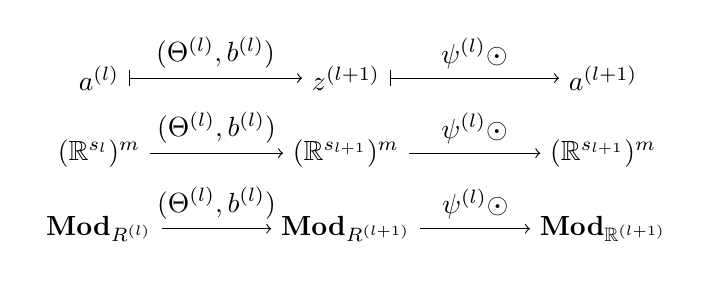
\begin{tikzpicture}
  \matrix (m) [matrix of math nodes, row sep=1.1em, column sep=4em, minimum width=1em]
  {
a^{(l)} & z^{(l+1)} & a^{(l+1)} \\ 
(\mathbb{R}^{s_l})^m & (\mathbb{R}^{s_{l+1}})^m & (\mathbb{R}^{s_{l+1}})^m  \\ 
\text{\textbf{Mod}}_{R^{(l)}} & \text{\textbf{Mod}}_{R^{(l+1)}} & \text{\textbf{Mod}}_{\mathbb{R}^{(l+1)}} \\ 
};
  \path[|->]
  (m-1-1) edge node [above] {$(\Theta^{(l)}, b^{(l)})$} (m-1-2)
  (m-1-2) edge node [above] {$\psi^{(l)} \odot$ } (m-1-3)
  ;
\path[->]
  (m-2-1) edge node [above] {$(\Theta^{(l)}, b^{(l)})$} (m-2-2)
  (m-2-2) edge node [above] {$\psi^{(l)} \odot$ } (m-2-3)
  ;
\path[->]
  (m-3-1) edge node [above] {$(\Theta^{(l)}, b^{(l)})$} (m-3-2)
  (m-3-2) edge node [above] {$\psi^{(l)} \odot$ } (m-3-3)
  ;
\end{tikzpicture}
\end{equation}

Since we need to operate with the activation function $\psi^{(l)} \odot$ elementwise, we (implicitly) equip $\text{\textbf{Mod}}_{R^{(l+1)}}$ with the Hadamard product.  In fact, with composition, we can represent the $l$th axon as 
\begin{equation}
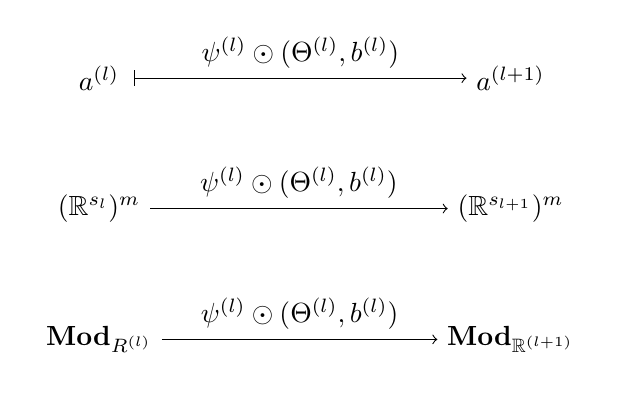
\begin{tikzpicture}
  \matrix (m) [matrix of math nodes, row sep=3.1em, column sep=10em, minimum width=2.5em]
  {
a^{(l)}  & a^{(l+1)} \\ 
(\mathbb{R}^{s_l})^m  & (\mathbb{R}^{s_{l+1}})^m  \\ 
\text{\textbf{Mod}}_{R^{(l)}}   & \text{\textbf{Mod}}_{\mathbb{R}^{(l+1)}} \\ 
};
  \path[|->]
  (m-1-1) edge node [above] {$\psi^{(l)} \odot (\Theta^{(l)}, b^{(l)})$} (m-1-2)
  ;
\path[->]
  (m-2-1) edge node [above] {$\psi^{(l)} \odot (\Theta^{(l)}, b^{(l)})$} (m-2-2)
  ;
\path[->]
  (m-3-1) edge node [above] {$\psi^{(l)} \odot (\Theta^{(l)}, b^{(l)})$} (m-3-2)
  ;
\end{tikzpicture} 
\end{equation}
The lesson is this: instead of thinking of layers, each separately, think of or focus on the relationship, the relations, between each layers, the axon, as one whole entity.  

Suppose we "feed in" input data $X$ into the first or $0$th layer of this NN.  This means that for $a^{(0)} \in \mathbb{R}^d$, 
\[
a^{(0)} = X^{(i)}
\]
for the $i$th (training) example.  

The "output" layer, layer $L$, should output the \emph{predicted} value, given $X$.  So 
\[
a^{(L)} \in \mathbb{R} \text{ or } \lbrace 0 ,1 , \dots K-1\rbrace \text{ or } [0,1]
\]
for regression, or classification (so it takes on discrete values) or the probability likelihood of being in some class $k$, respectively. 
 
The entire NN can mathematically expressed as follows: 
\begin{equation}
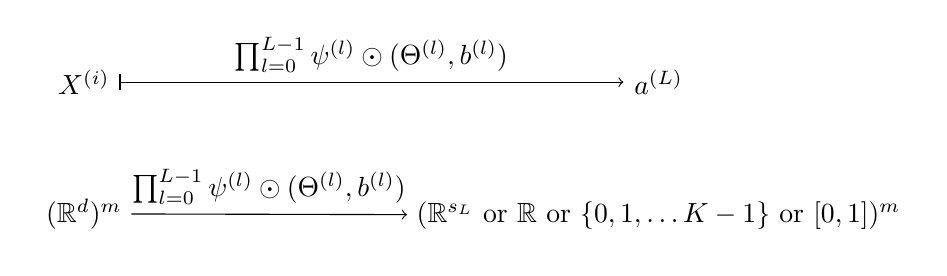
\begin{tikzpicture}
  \matrix (m) [matrix of math nodes, row sep=3.1em, column sep=10em, minimum width=2.5em]
  {
X^{(i)}  & a^{(L)} \\ 
(\mathbb{R}^{d})^m  & (\mathbb{R}^{s_L} \text{ or } \mathbb{R} \text{ or } \lbrace 0 ,1,\dots K-1\rbrace \text{ or } [0,1])^m  \\ 
};
  \path[|->]
  (m-1-1) edge node [above] {$\prod_{l=0}^{L-1} \psi^{(l)} \odot (\Theta^{(l)}, b^{(l)})$} (m-1-2)
  ;
\path[->]
  (m-2-1) edge node [above] {$\prod_{l=0}^{L-1} \psi^{(l)} \odot (\Theta^{(l)}, b^{(l)})$} (m-2-2)
  ;
\end{tikzpicture} 
\end{equation}





\begin{thebibliography}{9}


  
\end{thebibliography}



\end{document}
